% Compile (local):
%   pdflatex TECHNICAL_REPORT.tex
%   pdflatex TECHNICAL_REPORT.tex
% Windows: install MiKTeX or TeX Live and ensure `pdflatex` is on PATH.
% Online: upload TECHNICAL_REPORT.tex to Overleaf (Menu -> Compiler: pdfLaTeX).
% Figures live in ./figures/ (PNG). Upload the whole figures/ directory with this .tex to Overleaf.

\documentclass[11pt,letterpaper]{article}

\usepackage[utf8]{inputenc}
\usepackage[T1]{fontenc}
\usepackage{lmodern}
\usepackage[margin=1in]{geometry}
\usepackage{graphicx}
\usepackage{booktabs}
\usepackage{longtable}
\usepackage{array}
\usepackage{hyperref}
\usepackage{xcolor}
\usepackage{listings}
\usepackage{caption}
\usepackage{enumitem}
\usepackage{parskip}
\usepackage{fancyvrb}

\hypersetup{
  colorlinks=true,
  linkcolor=blue!60!black,
  urlcolor=blue!70!black,
  citecolor=blue!60!black,
  pdftitle={FightForge Technical Report},
  pdfauthor={Craig Omozeje, Tucker Ambrose}
}

\lstdefinelanguage{JavaScript}{
  keywords={async, await, break, case, catch, const, continue, debugger, default, delete, do, else, export, false, finally, for, function, if, import, in, instanceof, let, new, null, return, switch, this, throw, true, try, typeof, var, void, while, with, yield, class, extends},
  sensitive=true,
  comment=[l]{//},
  morecomment=[s]{/*}{*/},
  morestring=[b]',
  morestring=[b]"
}
\lstset{
  basicstyle=\ttfamily\small,
  keywordstyle=\color{blue!70!black}\bfseries,
  commentstyle=\color{gray!60}\itshape,
  stringstyle=\color{green!40!black},
  breaklines=true,
  frame=single,
  frameround=tttt,
  columns=fullflexible,
  showstringspaces=false,
  tabsize=2
}

\title{\vspace{-2em}\Large\textbf{SE/COM S 3190} --- Construction of User Interfaces\\[0.8em]
\LARGE Final Project Technical Report\\[0.3em]
\large Spring 2026}
\author{}
\date{}

\begin{document}

% ---------- Title page ----------
\begin{titlepage}
  \centering
  \vspace*{1.5cm}
  {\Large\bfseries SE/COM S 3190 --- Construction of User Interfaces\par}
  \vspace{0.6cm}
  {\LARGE\bfseries Final Project Technical Report\par}
  \vspace{0.4cm}
  {\large Spring 2026\par}
  \vspace{2cm}
  {\Huge\bfseries FightForge\par}
  \vspace{1.5cm}
  \begin{tabular}{p{2.8in}p{2.8in}}
    \textbf{Craig Omozeje} & \textbf{Tucker Ambrose} \\
    \texttt{comozeje@iastate.edu} & \texttt{tambrose@iastate.edu} \\
  \end{tabular}\\[0.8em]
  {\small\textit{Confirm Iowa State email addresses match your netIDs before submitting.}\par}
  \vfill
  {\large Iowa State University\par}
  {\large Department of Computer Science\par}
  \vspace{1.5cm}
\end{titlepage}

\tableofcontents
\newpage

% =============================================================================
\section{Introduction}

\subsection{Project overview}
\textbf{Problem statement.} Athletes and coaches need a single place to coordinate training plans, nutrition, progress metrics, and communication. Spreadsheets, group chats, and ad hoc documents are easy to lose and do not map well to roles (athlete vs.\ coach vs.\ admin).

\textbf{Relevance.} Clear assignment of workouts and meals, visible progress over time, and role-based access reduce friction for gyms, camps, and remote coaching.

\textbf{What FightForge does.} FightForge is a \textbf{web application} with a React (Vite) frontend and an Express.js REST API backed by \textbf{MySQL}. Users sign up or log in, receive a JWT, and access dashboards and CRUD-style features according to their role (\texttt{athlete}, \texttt{coach}, or \texttt{admin}).

\textbf{Scope.} Full-stack SPA: authentication, dashboards, workouts, meal plans, progress charts, messaging, friends/leaderboards, profile with JSON-stored preferences, and curated libraries for workouts and meals.

\subsection{Target users and use cases}
\textbf{Primary users --- athletes}
\begin{itemize}[nosep]
  \item Log in, view assigned workouts and meals, mark items complete, log body metrics, chat with a coach, and compare progress with friends on a leaderboard.
\end{itemize}

\textbf{Primary users --- coaches}
\begin{itemize}[nosep]
  \item View athletes linked via \texttt{coach\_id}, create/update/delete workouts and meals for those athletes, use generators and library copy flows, and message athletes.
\end{itemize}

\textbf{Secondary users --- admins}
\begin{itemize}[nosep]
  \item Broader visibility (e.g., workout lists across users in API logic) and an admin home route in the UI.
\end{itemize}

\textbf{Typical workflows}
\begin{enumerate}[nosep]
  \item Athlete completes signup $\rightarrow$ lands on athlete dashboard $\rightarrow$ opens Workouts $\rightarrow$ completes a session (XP may update).
  \item Coach logs in $\rightarrow$ coach home $\rightarrow$ manages plans for assigned athletes.
  \item Two athletes exchange friend requests $\rightarrow$ accept $\rightarrow$ leaderboard reflects accepted friendships.
\end{enumerate}

\subsection{Core features}
\begin{itemize}[nosep]
  \item \textbf{Authentication:} Signup, login, JWT in \texttt{Authorization} header; protected routes on client and \texttt{authenticate} middleware on server.
  \item \textbf{Workouts \& library:} CRUD on \texttt{workouts}, browse \texttt{workout\_library}, copy templates, generate plans, mark complete (ties into XP in \texttt{lib/xp.js}).
  \item \textbf{Meals \& meal library:} Similar patterns for \texttt{meals} / \texttt{meal\_library}.
  \item \textbf{Progress:} CRUD-style entries in \texttt{progress\_entries} with chart-friendly data.
  \item \textbf{Messages:} Threaded messaging with read/saved semantics per schema.
  \item \textbf{Friends:} \texttt{friendships} with \texttt{pending} / \texttt{accepted} states.
  \item \textbf{Profile:} JSON \texttt{profile} on \texttt{users}, avatar as data URL (size limits enforced in routes).
  \item \textbf{Role-based UI:} \texttt{App.jsx} gates \texttt{/dashboard}, \texttt{/coach}, and \texttt{/admin} using \texttt{ProtectedRoute} and role checks.
\end{itemize}

\subsection{Originality vs.\ inspiration}
FightForge is \textbf{inspired by} sports camp and combat-sports training platforms (training logs, macros, messaging), built as an \textbf{open-source} full-stack application. Bundled \textbf{sample accounts} (\texttt{@fightforge.test}) and seed data exist for \textbf{local development only}; production should use real signups and rotated credentials. The app includes a \textbf{progression-style} XP/overall model (see schema comments) and \textbf{ephemeral messaging} in \texttt{schema.sql} (lazy cleanup after read unless saved).

% =============================================================================
\section{System overview and project description}

\subsection{Major functional modules}
\begin{longtable}{@{}p{1.9in}p{4.6in}@{}}
  \toprule
  \textbf{Module} & \textbf{Responsibility} \\
  \midrule
  \endhead
  \textbf{Auth} (\texttt{routes/auth.js}, \texttt{middleware/auth.js}) & Signup/login, JWT sign/verify, profile-by-id with authorization rules. \\
  \textbf{Users} (\texttt{routes/users.js}) & Profile updates, avatars, coach assignment where applicable. \\
  \textbf{Workouts} (\texttt{routes/workouts.js}, \texttt{lib/planGenerators.js}) & List/filter by role, CRUD, library, generation, completion + XP. \\
  \textbf{Meals} (\texttt{routes/meals.js}) & Meal CRUD and library/generation patterns. \\
  \textbf{Progress} (\texttt{routes/progress.js}) & Entries per user over time. \\
  \textbf{Messages} (\texttt{routes/messages.js}) & Send/list/mark read/save. \\
  \textbf{Friends} (\texttt{routes/friends.js}) & Requests, accept, leaderboard data. \\
  \textbf{API shell} (\texttt{server.js}) & CORS, JSON body parsing, JSON parse error handling, route mounting, 404 + global error handler. \\
  \textbf{Frontend shell} (\texttt{App.jsx}, \texttt{AppShell.jsx}, \texttt{AuthContext.jsx}) & Router, auth provider, layout, \texttt{apiFetch} wrapper. \\
  \bottomrule
\end{longtable}

Modules communicate over \textbf{HTTP/JSON}; the database is the shared persistence layer via \texttt{mysql2} pool (\texttt{config/db.js}).

\subsection{UI and navigation flow}
\begin{enumerate}[nosep]
  \item \textbf{Public:} \texttt{/} (Home), \texttt{/login}, \texttt{/signup}.
  \item \textbf{Authenticated (inside \texttt{AppShell}):}
    \begin{itemize}[nosep]
      \item Athlete: \texttt{/dashboard}, \texttt{/workouts}, \texttt{/workouts/library}, \texttt{/progress}, \texttt{/meals}, \texttt{/chat}, \texttt{/profile}, \texttt{/friends}.
      \item Coach (non-athlete): \texttt{/coach} and same shell routes as permitted by UI/API.
      \item Admin: \texttt{/admin} (admin-only gate).
    \end{itemize}
  \item \textbf{Gates:} \texttt{AthleteDashboardGate} redirects coaches/admins away from \texttt{/dashboard}; \texttt{CoachOrAdminGate} keeps athletes off \texttt{/coach}; \texttt{AdminOnlyGate} restricts \texttt{/admin}.
\end{enumerate}

\subsection{CRUD entities}
The MySQL schema in \texttt{backend/database/schema.sql} defines the main entities. Summary:

\begin{longtable}{@{}p{1.15in}p{2.05in}p{3.2in}@{}}
  \toprule
  \textbf{Entity} & \textbf{Key fields (abbrev.)} & \textbf{CRUD / actions} \\
  \midrule
  \endhead
  \textbf{users} & email, password\_hash, full\_name, role, coach\_id, profile (JSON), avatar\_url, xp, overall & Create via signup; read/update via users + auth profile routes; delete not emphasized in UI (cascade via FKs). \\
  \textbf{workouts} & title, description, content, video\_url, athlete\_id, created\_by, completed\_at & Full CRUD via API for coaches/admins; athletes read and may complete. \\
  \textbf{meals} & title, description, macros, notes, athlete\_id, created\_by, completed\_at & Same pattern as workouts. \\
  \textbf{progress\_entries} & user\_id, metrics, recorded\_at & Create/read/update/delete per progress routes. \\
  \textbf{messages} & sender\_id, recipient\_id, body, seen\_at, saved & Create + read + state updates. \\
  \textbf{friendships} & requester\_id, recipient\_id, status & Create (request), update (accept), read for leaderboard. \\
  \textbf{workout\_library / meal\_library} & Template metadata & Read-heavy; copy/insert into user-specific rows via API. \\
  \bottomrule
\end{longtable}

Relationships include \textbf{users $\rightarrow$ users} (\texttt{coach\_id}), \textbf{workouts/meals $\rightarrow$ users} (athlete and creator), \textbf{progress\_entries $\rightarrow$ users}, \textbf{messages} between users, and \textbf{friendships} between users. Indexes on foreign keys and common filters are declared at the end of \texttt{schema.sql}.

% =============================================================================
\section{File and folder architecture}

\subsection{Folder structure overview}
The repository uses \textbf{\texttt{frontend/}} and \textbf{\texttt{backend/}} at the project root. This separation keeps Node dependencies, build tooling (Vite), and API deployment (Express, MySQL) independent, avoids leaking server-only secrets into the client bundle, and matches common industry practice for SPAs + REST APIs.

\subsection{Backend folder structure}
\subsubsection{Backend folder tree}
\begin{figure}[htbp]
  \centering
  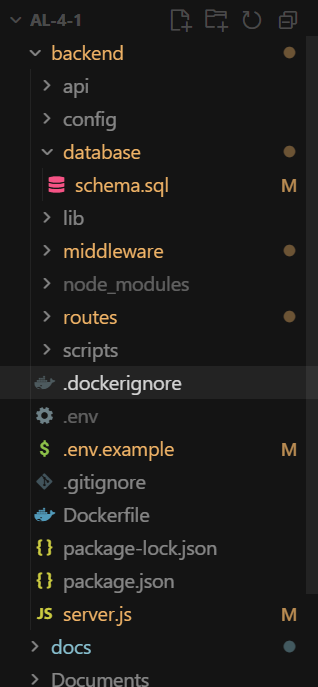
\includegraphics[width=0.95\textwidth,keepaspectratio]{figures/backend-tree.png}
  \caption{Repository and \texttt{backend/} folder structure in the IDE.}
\end{figure}

\noindent Textual summary:

\begin{Verbatim}[fontsize=\small]
backend/
├── config/           db.js (MySQL pool)
├── database/         schema.sql
├── lib/              planGenerators.js, xp.js
├── middleware/       auth.js
├── routes/           auth, users, workouts, meals, progress, messages, friends
├── scripts/          seed.js
├── server.js
├── package.json
├── Dockerfile, .env.example
└── api/              (placeholder / future use)
\end{Verbatim}

\subsubsection{Backend folder description}
\begin{itemize}[nosep]
  \item \textbf{\texttt{config/db.js}} --- Creates a \texttt{mysql2/promise} pool from \texttt{DB\_*} environment variables.
  \item \textbf{\texttt{routes/*.js}} --- One Express router per domain; mounted under \texttt{/api/...} in \texttt{server.js}.
  \item \textbf{\texttt{middleware/auth.js}} --- JWT verification and \texttt{requireRole}.
  \item \textbf{\texttt{lib/}} --- Pure helpers (plan generation, XP awards) to keep route files smaller.
  \item \textbf{\texttt{database/schema.sql}} --- Source of truth for tables, FKs, and indexes.
  \item \textbf{\texttt{scripts/seed.js}} --- Optional sample users and library data after schema load.
\end{itemize}

\subsection{Frontend folder structure}
\subsubsection{Frontend folder tree}
\begin{figure}[htbp]
  \centering
  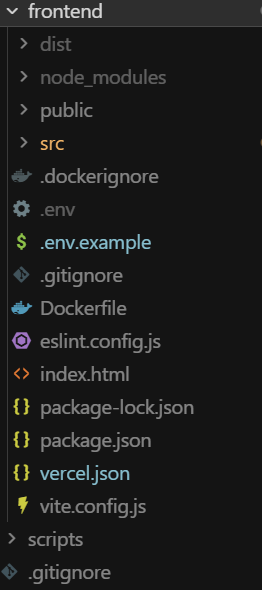
\includegraphics[width=0.95\textwidth,keepaspectratio]{figures/frontend-tree.png}
  \caption{\texttt{frontend/} project layout (Vite, Docker, ESLint, Vercel config).}
\end{figure}

\noindent Summary:

\begin{Verbatim}[fontsize=\small]
frontend/src/
├── api/client.js       buildUrl, apiFetch, token helpers
├── components/         AppShell, ProtectedRoute, Modal, Avatar, Charts, YouTubePlayer, Icon
├── context/            AuthContext.jsx
├── pages/              Home, Login, Signup, Dashboard, Workouts, WorkoutLibrary,
│                       Progress, Meals, Chat, Profile, Friends, CoachHome, AdminHome, NotFound
├── utils/              image.js, youtube.js
├── config.js           feature flags (e.g.\ optional sample-account UI)
├── App.jsx, main.jsx, index.css
└── assets/
\end{Verbatim}

\subsubsection{Frontend folder description}
\begin{itemize}[nosep]
  \item \textbf{\texttt{pages/}} --- Route-level views; each major screen has a \texttt{.jsx} and often a colocated \texttt{.css}.
  \item \textbf{\texttt{components/}} --- Reusable UI (layout shell, modals, charts, video).
  \item \textbf{\texttt{context/AuthContext.jsx}} --- Holds user state and wraps \texttt{login} / \texttt{logout} / \texttt{refreshProfile} around \texttt{apiFetch}.
  \item \textbf{\texttt{api/client.js}} --- Centralizes \texttt{fetch}, JWT header, and error parsing so pages stay declarative.
\end{itemize}

% =============================================================================
\section{Code explanation and logic flow}

\subsection{Frontend--backend interaction}
\begin{enumerate}[nosep]
  \item \textbf{\texttt{apiFetch(path, \{ method, body, token \})}} (\texttt{frontend/src/api/client.js}) builds the URL: in dev, paths like \texttt{/api/...} stay relative so \textbf{Vite's proxy} forwards them to \texttt{VITE\_PROXY\_TARGET} (default \texttt{http://127.0.0.1:5000}); in production, \texttt{VITE\_API\_BASE} prefixes the absolute API host.
  \item \textbf{JSON bodies} are sent with \texttt{Content-Type: application/json} for POST/PUT-style calls.
  \item \textbf{Responses} are parsed as JSON when possible; failures throw an \texttt{Error} whose \texttt{message} comes from \texttt{data.error}, \texttt{data.message}, or \texttt{res.statusText}.
  \item \textbf{UI error handling} --- e.g.\ \texttt{Login.jsx} uses \texttt{try/catch} on \texttt{login()} and sets local error state for an alert paragraph.
\end{enumerate}

\subsection{React component example (Login)}
\texttt{Login.jsx} implements the sign-in form: controlled inputs for email/password, \texttt{loading} state to disable the submit button, role-based redirect after success, and optional sample-account quick-fill when \texttt{VITE\_SHOW\_DEMO\_ACCOUNTS} is true.

\begin{lstlisting}[language=JavaScript,caption={Excerpt from \texttt{frontend/src/pages/Login.jsx} (submit handler)}]
async function onSubmit(e) {
  e.preventDefault();
  setError('');
  setLoading(true);
  try {
    await login(email, password);
  } catch (err) {
    setError(err.message || 'Login failed');
  } finally {
    setLoading(false);
  }
}
\end{lstlisting}

\texttt{login} comes from \texttt{AuthContext} and calls \texttt{apiFetch('/api/auth/login', \{ method: 'POST', body: \{ email, password \}, token: null \})}, then stores the JWT and user in \texttt{localStorage}.

\subsection{API route examples (workouts)}
All workout routes live under \textbf{\texttt{/api/workouts}} with \textbf{\texttt{authenticate}} middleware. Examples:

\begin{longtable}{@{}llp{3.5in}@{}}
  \toprule
  \textbf{Verb} & \textbf{Path} & \textbf{Purpose} \\
  \midrule
  \endhead
  GET & \texttt{/api/workouts} & List workouts; SQL varies by admin / coach / athlete (see \texttt{routes/workouts.js}). \\
  POST & \texttt{/api/workouts} & \textbf{Create} workout (coach/admin); body includes \texttt{title}, \texttt{athleteId}, optional \texttt{description}, \texttt{content}, \texttt{videoUrl}. Validates athlete exists and coach owns athlete when applicable; \textbf{201} + JSON row. \\
  PUT & \texttt{/api/workouts/:id} & \textbf{Update} workout fields; dynamic \texttt{UPDATE} from provided body keys; \textbf{403} if not allowed, \textbf{404} if missing. \\
  DELETE & \texttt{/api/workouts/:id} & \textbf{Delete} workout; \textbf{204} on success. \\
  \bottomrule
\end{longtable}

Errors generally return JSON \texttt{\{ error: string \}} with \textbf{4xx/5xx} as appropriate; unexpected exceptions log server-side and return \textbf{500}.

\subsection{Database interaction}
\begin{itemize}[nosep]
  \item \textbf{Engine:} MySQL (InnoDB), UTF-8MB4.
  \item \textbf{Types \& constraints:} \texttt{ENUM} for roles and related enums, \texttt{JSON} for flexible athlete profile, \texttt{FOREIGN KEY} with \texttt{ON DELETE CASCADE} where orphan rows must not remain.
  \item \textbf{Indexing:} e.g.\ \texttt{idx\_workouts\_athlete}, \texttt{idx\_messages\_pair}, friendship indexes --- support common filters without full table scans as data grows.
  \item \textbf{Typical access:} Parameterized queries via \texttt{pool.query('... ? ...', [params])} to mitigate SQL injection.
\end{itemize}

% =============================================================================
\section{Screenshots and web views}
Screenshots below show the FightForge athlete experience (local dev at \texttt{localhost:5173}) and key nutrition, progress, social, and messaging views.

\begin{figure}[htbp]
  \centering
  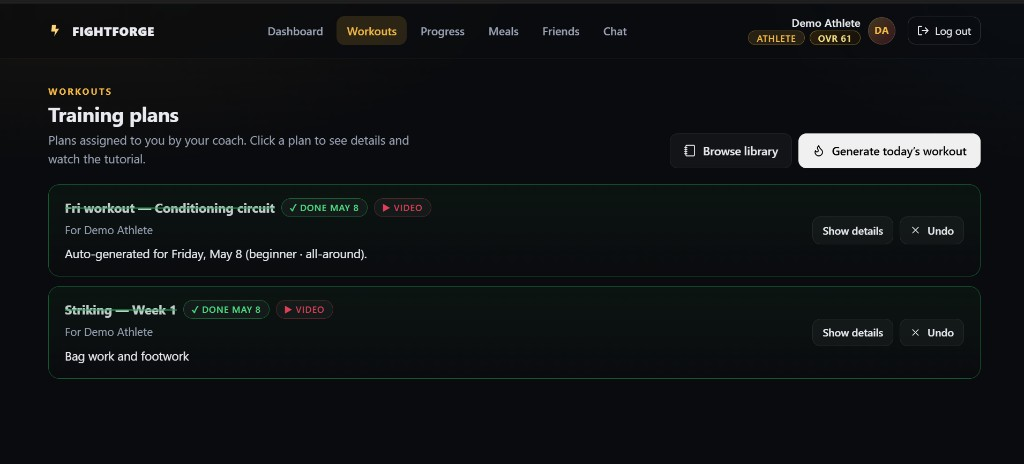
\includegraphics[width=0.95\textwidth,keepaspectratio]{figures/workouts.png}
  \caption{Workouts --- training plans assigned to the athlete (completed plans, video links, generate/browse actions).}
\end{figure}

\begin{figure}[htbp]
  \centering
  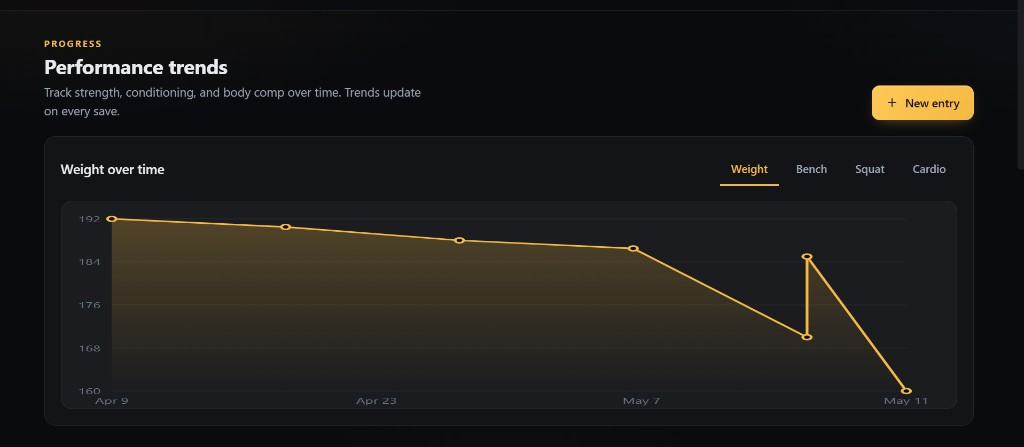
\includegraphics[width=0.95\textwidth,keepaspectratio]{figures/progress.png}
  \caption{Progress --- performance trends; weight over time with tabbed metrics (bench, squat, cardio).}
\end{figure}

\begin{figure}[htbp]
  \centering
  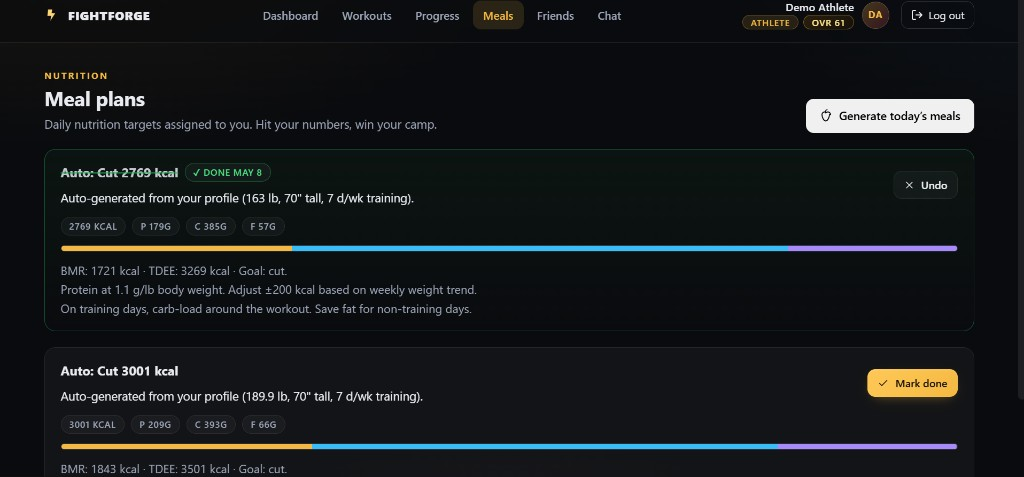
\includegraphics[width=0.95\textwidth,keepaspectratio]{figures/meals.png}
  \caption{Meals --- daily nutrition targets, macro breakdown, BMR/TDEE, and mark-done flow.}
\end{figure}

\begin{figure}[htbp]
  \centering
  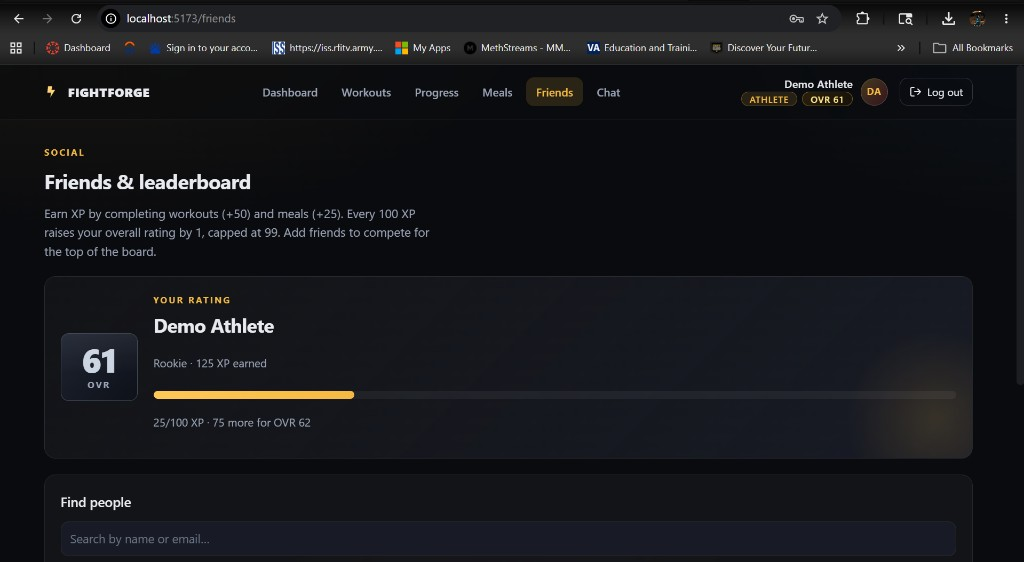
\includegraphics[width=0.95\textwidth,keepaspectratio]{figures/friends.png}
  \caption{Friends --- leaderboard, XP/OVR card, and find-people search.}
\end{figure}

\begin{figure}[htbp]
  \centering
  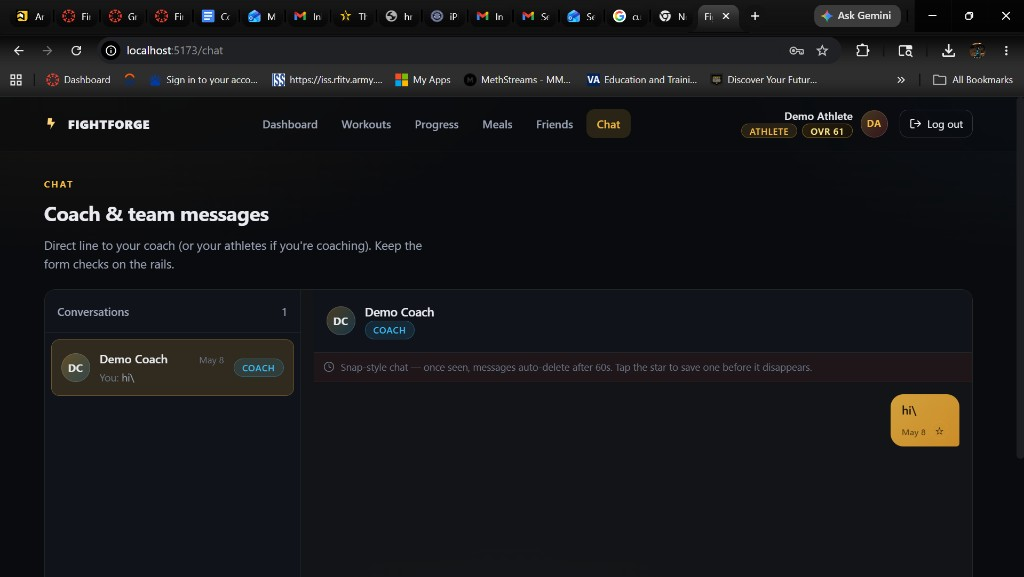
\includegraphics[width=0.95\textwidth,keepaspectratio]{figures/chat.png}
  \caption{Chat --- coach/athlete messaging, conversation list, and ephemeral (Snap-style) save hint.}
\end{figure}

% =============================================================================
\section{Installation and setup instructions}

\subsection{Frontend setup}
\begin{itemize}[nosep]
  \item \textbf{Node:} Use a current LTS (project uses Vite 5 and React 19; \textbf{Node 18+} recommended).
  \item \textbf{Install:} \texttt{cd frontend} then \texttt{npm install}.
  \item \textbf{Environment:} Copy \texttt{frontend/.env.example} to \texttt{frontend/.env}. For local dev, leave \texttt{VITE\_API\_BASE} empty so \texttt{/api} is proxied; set \texttt{VITE\_PROXY\_TARGET} if the API is not on port 5000.
  \item \textbf{Run:} \texttt{npm run dev} --- Vite prints a local URL (often port \textbf{5173}).
  \item \textbf{Build:} \texttt{npm run build} then \texttt{npm run preview} to test production bundle locally.
\end{itemize}

\subsection{Backend setup}
\begin{itemize}[nosep]
  \item \textbf{Node:} \textbf{18+} recommended (same as frontend).
  \item \textbf{Install:} \texttt{cd backend} then \texttt{npm install}.
  \item \textbf{Run:} \texttt{npm start} or \texttt{node server.js} (see \texttt{backend/package.json}). Default port \textbf{5000} unless \texttt{PORT} is set.
  \item \textbf{Seed (optional):} After DB is ready, \texttt{npm run seed} runs \texttt{scripts/seed.js} (sample password printed to the console).
\end{itemize}

\subsection{Database setup}
\begin{itemize}[nosep]
  \item \textbf{System:} \textbf{MySQL} (local or hosted).
  \item \textbf{Create schema:} e.g.\ \texttt{mysql -u root -p < backend/database/schema.sql} (adjust user/host; on Windows, MySQL Workbench can run the file).
  \item \textbf{Seed:} \texttt{cd backend \&\& npm run seed}
  \item \textbf{Connection:} Set \texttt{DB\_HOST}, \texttt{DB\_PORT}, \texttt{DB\_USER}, \texttt{DB\_PASSWORD}, \texttt{DB\_NAME} in \texttt{backend/.env} (see \texttt{.env.example}).
\end{itemize}

\subsection{Environment variables}
\textbf{Backend} (\texttt{backend/.env.example} as reference)

\begin{longtable}{@{}p{2.4in}p{3.9in}@{}}
  \toprule
  \textbf{Variable} & \textbf{Purpose} \\
  \midrule
  \endhead
  \texttt{PORT} & API listen port \\
  \texttt{DB\_HOST}, \texttt{DB\_PORT}, \texttt{DB\_USER}, \texttt{DB\_PASSWORD}, \texttt{DB\_NAME} & MySQL connection \\
  \texttt{JWT\_SECRET} & Signing key for JWTs (strong value required in production; see \texttt{server.js}) \\
  \texttt{CORS\_ORIGIN} & Comma-separated allowed browser origins in \textbf{production} when set (see \texttt{server.js} logic) \\
  \texttt{NODE\_ENV} & Set to \texttt{production} for production hardening \\
  \bottomrule
\end{longtable}

\textbf{Frontend} (\texttt{frontend/.env.example})

\begin{longtable}{@{}p{2.4in}p{3.9in}@{}}
  \toprule
  \textbf{Variable} & \textbf{Purpose} \\
  \midrule
  \endhead
  \texttt{VITE\_API\_BASE} & Absolute API base in production builds (empty in local dev) \\
  \texttt{VITE\_PROXY\_TARGET} & Dev-only proxy target for \texttt{/api} \\
  \texttt{VITE\_SHOW\_DEMO\_ACCOUNTS} & Optional sample-account quick-fill (keep \texttt{false} in production) \\
  \bottomrule
\end{longtable}

% =============================================================================
\section{Contribution overview}

\subsection{Craig Omozeje --- contributions}
Craig delivered \textbf{the majority of the full-stack application}---backend, database, integration, and most of the React UI.

\begin{itemize}[nosep]
  \item \textbf{Express API:} Implemented and maintained \texttt{routes/workouts.js}, \texttt{routes/meals.js}, \texttt{routes/progress.js}, \texttt{routes/messages.js}, \texttt{routes/friends.js}, and \texttt{routes/users.js}; integrated \texttt{lib/planGenerators.js} and \texttt{lib/xp.js} for generated plans and XP on workout completion.
  \item \textbf{Auth \& platform:} \texttt{routes/auth.js} (signup, login, profile access rules), \texttt{middleware/auth.js} (JWT verify, \texttt{requireRole}), and mounting in \texttt{server.js}.
  \item \textbf{Server \& ops:} \texttt{server.js} --- CORS (environment-aware), JSON body limits, JSON parse error middleware (400), global error handler, health route; \texttt{backend/.env.example}, Dockerfile, and local run documentation.
  \item \textbf{Database:} \texttt{database/schema.sql} (all tables, FKs, indexes) and \texttt{scripts/seed.js} for optional sample accounts and starter camp data; \texttt{config/db.js} MySQL pool.
  \item \textbf{Frontend (React / Vite):} \texttt{App.jsx} (routes, role gates), \texttt{main.jsx}, \texttt{AuthContext.jsx}, \texttt{api/client.js}, \texttt{config.js}; pages including \texttt{Home.jsx}, \texttt{Login.jsx}, \texttt{Signup.jsx}, \texttt{Dashboard.jsx}, \texttt{Workouts.jsx}, \texttt{WorkoutLibrary.jsx}, \texttt{Progress.jsx}, \texttt{Meals.jsx}, \texttt{Chat.jsx}, \texttt{Profile.jsx}, \texttt{Friends.jsx}, \texttt{CoachHome.jsx}, \texttt{AdminHome.jsx}, \texttt{NotFound.jsx}; layout and components such as \texttt{AppShell.jsx}, \texttt{ProtectedRoute.jsx}, \texttt{Modal.jsx}, \texttt{Avatar.jsx}, \texttt{Charts.jsx}, \texttt{YouTubePlayer.jsx}, \texttt{Icon.jsx}; shared styles (\texttt{index.css}, \texttt{pageLayout.css}, page-specific CSS).
  \item \textbf{Utilities:} \texttt{utils/youtube.js}, \texttt{utils/image.js} where used for media and profile flows.
  \item \textbf{Documentation:} Primary author of this technical report (structure, installation, architecture, code explanation).
\end{itemize}

\subsection{Tucker Ambrose --- contributions}

% =============================================================================
\section{Challenges faced}

\subsection{Craig Omozeje --- challenges}
\textbf{Challenge A --- Login failures surfaced as generic 500.}\\
\textbf{Root cause:} Strict \texttt{CORS\_ORIGIN} did not always match the browser's real \texttt{Origin} (e.g.\ \texttt{localhost} vs.\ \texttt{127.0.0.1}, or Vite ``Network'' URLs), and an earlier pattern passed \texttt{Error} into the \texttt{cors} callback, which Express routed to the global error handler.\\
\textbf{Diagnosis:} Reproduced with DevTools Network (failed preflight or opaque errors), read \texttt{server.js} and \texttt{cors} internals, and compared working \texttt{curl} vs.\ browser requests.\\
\textbf{Solution:} Environment-aware CORS (\texttt{origin: true} in non-production; strict allowlist only when \texttt{NODE\_ENV=production} and \texttt{CORS\_ORIGIN} is set), never pass \texttt{Error} for policy deny, JSON body parse middleware returning 400, and a guard on \texttt{password\_hash} before \texttt{bcrypt.compare} in \texttt{routes/auth.js}.\\
\textbf{Learning:} CORS and credentials are part of the API contract; test from the actual browser origin, not only from CLI.

\vspace{0.6em}
\textbf{Challenge B --- XP drift when toggling workout completion.}\\
\textbf{Root cause:} Double-clicks and race conditions could apply XP twice or revert inconsistently if completion timestamps and XP updates were not treated as one logical unit.\\
\textbf{Diagnosis:} Logged \texttt{completed\_at} before/after in MySQL and traced \texttt{awardXp} in \texttt{lib/xp.js} from \texttt{POST /api/workouts/:id/complete}.\\
\textbf{Solution:} Tightened the handler so XP is awarded only on transitions into ``complete'' from incomplete (and reversed only when undoing), with server-side checks on prior state.\\
\textbf{Learning:} Idempotency matters for ``toggle'' style endpoints in production APIs.

\vspace{0.6em}
\textbf{Challenge C --- Layout shift when embedding YouTube.}\\
\textbf{Root cause:} iframe aspect ratio was not reserved before load, so cards jumped when the player mounted.\\
\textbf{Diagnosis:} Chrome Layout Instability tooling and throttled network testing.\\
\textbf{Solution:} Fixed aspect-ratio wrapper in CSS around \texttt{YouTubePlayer} and deferred control chrome until \texttt{onLoad}.\\
\textbf{Learning:} Reserve space for async media up front.

\vspace{0.6em}
\textbf{Challenge D --- Friends leaderboard showed stale XP.}\\
\textbf{Root cause:} Client state did not refetch after workouts were completed on another view.\\
\textbf{Diagnosis:} Network tab timestamps vs.\ UI.\\
\textbf{Solution:} Refetch friends/leaderboard on relevant navigation and window focus, with a calmer loading state to avoid rank flicker.\\
\textbf{Learning:} Cross-page metrics need an explicit refresh strategy, not one-off local state.

\subsection{Tucker Ambrose --- challenges}

% =============================================================================
\section{Final reflections}

\subsection{Craig Omozeje --- reflection}
Carrying \textbf{most of the stack} meant context-switching between \textbf{MySQL}, \textbf{Express}, and \textbf{React} daily. I am much more confident in \textbf{JWT auth}, \textbf{role-based routing}, \textbf{REST design}, and \textbf{component-level UI} than at the start of the term. The most rewarding part was end-to-end ownership---from schema and seed data to dashboards and charts---so FightForge felt like one coherent product. If I started over, I would add a \textbf{shared API contract} (e.g.\ OpenAPI or typed DTOs) on day one to reduce camelCase/snake\_case drift between \texttt{apiFetch} bodies and SQL column names. I also learned to \textbf{reproduce issues in the browser first} (CORS, preflight, status codes) before blaming the database---skills that map directly to internships and small-team shipping.

\subsection{Tucker Ambrose --- reflection}

\vfill
\noindent\rule{\textwidth}{0.4pt}\\[0.3em]
\small\textit{This document follows the section structure of the SE/COM S 3190 Final Project Technical Report template (Spring 2026). PDF built from \texttt{TECHNICAL\_REPORT.tex} with figures in \texttt{figures/}. Upload \texttt{TECHNICAL\_REPORT.tex} and the \texttt{figures/} folder together to Overleaf or compile locally with \texttt{pdflatex}.}

\end{document}
